\documentclass[a4paper,11pt]{report}

\usepackage{amsmath}
\usepackage{fullpage}
\usepackage{graphicx}
\usepackage{hyperref}

\setlength{\parindent}{0pt}
\date{\today}

\begin{document}

\begin{center}
  \large{
    Pattern Recognition\\
    Spring 2019
  }
  
  \noindent\makebox[\linewidth]{\rule{\linewidth}{0.4pt}}
  Final report
  \noindent\makebox[\linewidth]{\rule{\linewidth}{0.4pt}}

  \begin{flushleft}
    Authors : Nicolas Fuchs, Jérôme Vonlanthen, Thomas Schaller and Sylvain Julmy
  \end{flushleft}

  
  % \noindent\makebox[\linewidth]{\rule{\linewidth}{0.4pt}}

  \noindent\makebox[\linewidth]{\rule{\textwidth}{1pt}}
\end{center}

\section*{Group Organization}

\section*{Tasks}

\subsection*{SVM}

The SVM task was achieved by using the
sklearn\footnote{\url{https://scikit-learn.org/stable/modules/svm.html}}
library, which is very simple to use and provides a lot of examples for a better
understanding.

In order to find the best parameter, we used a grid search approach with various
parameters and display the heatmaps of the results for each tested kernel (see below).

\begin{minipage}{0.49\textwidth}
  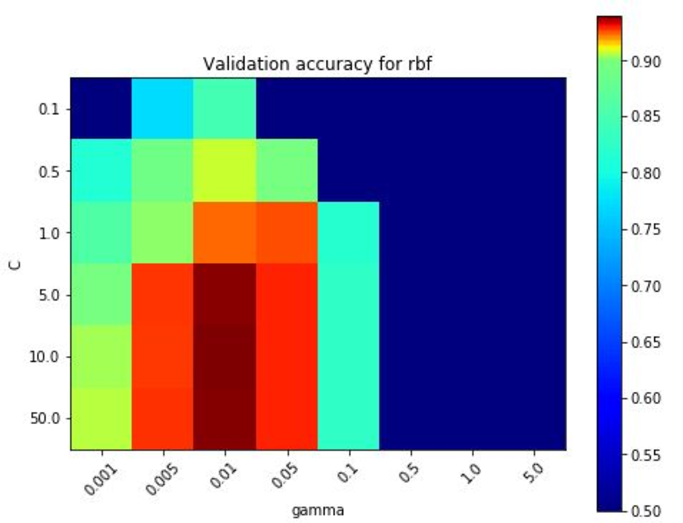
\includegraphics[width=0.8\textwidth]{figures/hm1.pdf}
\end{minipage}
\hfill
\begin{minipage}{0.49\textwidth}
  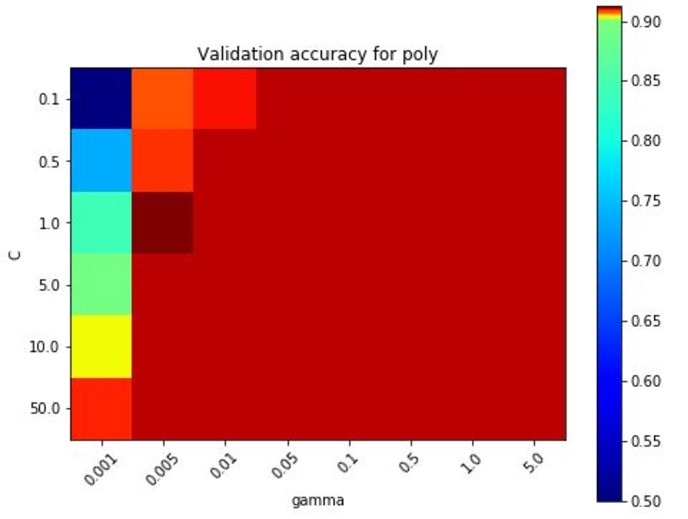
\includegraphics[width=0.8\textwidth]{figures/hm2.pdf}
\end{minipage}

Using this, we were able to obtain a $97.9\%$ accuracy.

\subsection*{MLP}

\subsection*{CNN}

\subsection*{Keyword spotting}

\subsection*{Signature Verification}

\section*{General thoughts and and feedback}

\end{document}